\documentclass[12pt]{article}

\usepackage{fullpage}
\usepackage{epsfig}
\usepackage{graphicx}

\newcommand{\code}[1]{\texttt{#1}}

\author{Marc G. Bellemare, Adam White, Mike Sokolsky}
\title{The RLAI Robotic Simulator\\ A Tutorial}

\begin{document}
\maketitle

\section{Introduction}

This tutorial documents the RL-Glue version of the RLAI Robotic Simulator: how 
to install it, how to run it and how to use it in your work. Included is a 
Standalone mode, where you can personally control the robot in the environment.
After performing the installation (Section \ref{sec:installation}),  I suggest 
running the simulator in Standalone mode (Section \ref{subsec:standalone}) 
once initially to get an idea of the environment in which the robot lives.

This tutorial is divided into four parts in ordering of increasing depth of
use. The first part is concerned with the actual simulator package - how
to install and run the simulator. The second part explains how to use the 
simulator, in particular how to write an agent and an RL environment. It
also discusses how to use one of the other pre-defined environments. The
third part details how to create new simulator environments (e.g. the 
constituent parts of the simulator, as opposed to the RL-specific aspects)
and how to modify existing objects and create new ones. The last part focuses
on adding functionality to the simulator, for example how to design new 
sensors or how to improve the physics engine.

\subsection{Notes}

Running the simulator requires the following:

\begin{itemize}
\item{Java 1.5}
\item{A POSIX operating system such as Mac OS X, Linux or BSD (for running the additonal scripts)}
item{RL-Glue Core 3.0}
\end{itemize}

This tutorial does not discuss RL-Glue, on which this version of the simulator
is based. For more information about RL-Glue, you are encouraged to visit:

\begin{verbatim}
http://glue.rl-community.org
\end{verbatim}

On there you will find a link to download the most recent version of the RL-Glue
core, which is needed to run the simulator. The simulator itself is based
on the RL-Glue Java codec. For ease of use, we distribute the codec along
with this simulator. However, users are encouraged to install the RL-Glue
Java codec if they plan on developing for the simulator. 

\section{Installing the RLAI Robotic Simulator}\label{sec:installation}

\subsection{Downloading the Package}

Each step of this section will be detailed with instructions for UNIX
systems. 

Along with this tutorial you should have downloaded a tarball of the 
RL-Glue version of the Simulator. If you have not yet done so, the Simulator
package can be found at

\begin{verbatim}
http://www.cs.ualberta.ca/~mg17/critterbot/files/RLGlueRLAISimulator.tgz
\end{verbatim}

For the remaining of this tutorial, I will assume that you have downloaded
this file to a directory called \verb+rlaisim+. Assuming that this 
is done, you should extract files from the tarball:

\begin{verbatim}
rlaisim> tar -xvzf RLAIRobotSimulator.tgz

<crunch crunch>

rlaisim> cd RLAIRobotSimulator
rlaisim/RLAIRobotSimulator>
\end{verbatim}

This will extract two directories, \code{RLGlueSim} and \code{example}.
The former contains the source for the abstract RL-Glue environment containing
the simulator; the latter contains example code that instantiates the
RL-Glue environment and provides a random agent and experiment.

\subsection{Building the RL-Glue Simulator Environment}

There are two parts to the RL-Glue Simulator Environment. The core part
encapsulates the RLAI Robotic Simulator into an abstract RL-Glue environment
which is then instantiated (the second part) into an environment with specific
action and observation spaces as well as a reward function.

In order to build the core environment and packaging it as a jar file, an
ant file has been provided:

\begin{verbatim}
rlaisim/RLAIRobotSimulator> cd RLGlueSim
rlaisim/RLAIRobotSimulator/RLGlueSim> ant build 

<crunch crunch>

BUILD SUCCESSFUL
Total time: 2 seconds
rlaisim/RLAIRobotSimulator/RLGlueSim>

\end{verbatim}

Provided everything went well, there should now be a file called RLGlueSim.jar
in the directory \code{RLGlueSim/products}. The next step is to copy it to
the example directory, so it can be used:

\begin{verbatim}
rlaisim/RLAIRobotSimulator/RLGlueSim> cp products/RLGlueSim.jar ../example/libs
\end{verbatim}

This completes the installation of the core RL-Glue simulator. The last
step is to return to the package root:

\begin{verbatim}
rlaisim/RLAIRobotSimulator/RLGlueSim> cd ..
rlaisim/RLAIRobotSimulator>
\end{verbatim}

\subsection{Running the Example}

With the package comes a full-fledged example containing an environment,
an agent (the random agent from the 
RL-Library\footnote{\code{http://rl-library.googlecode.com}}) and a 
sample experiment (also from the RL-Library). 

You should first ensure that the example code compiles. This can be done
by moving to the \code{example} directory and executing the script
\code{compile.sh}:

\begin{verbatim}
rlaisim/RLAIRobotSimulator> cd example
rlaisim/RLAIRobotSimulator/example> bash compile.sh

Compiled src/environment/DiscreteActionMapping.java src/environment/LightBasedRewardFunction.java src/environment/LightSensorsObservationMapping.java src/environment/SampleEnvironmentDescription.java src/environment/SampleSimulatorEnvironment.java src/environment/StandaloneSimulatorLoader.java
Compiled src/agent/RandomAgent.java
Compiled src/experiment/SampleExperiment.java

rlaisim/RLAIRobotSimulator/example>
\end{verbatim}

The script will warn you if compilation fails for some reason. Provided the
code does compile, you may either run the simulator in Standalone mode
(in which case you manually drive the robot) or run it via RL-Glue as a 
complete experiment.

\subsection{Running in Standalone Mode}\label{subsec:standalone}

The following will start the simulator in standalone mode:

\begin{verbatim}
rlaisim/RLAIRobotSimulator/example> bash runStandalone.sh 
\end{verbatim}

The \verb+runStandalone.sh+ script will compile the simulator loader,
\verb+src/environment/StandaloneSimulatorLoader.java+, and execute it. The 
specifics of this program will be detailed later in this tutorial.

Once you execute \verb+runStandalone.sh+, you should see a GUI appear, showing
the state of the simulator. The arrow keys will drive the robot around. Some 
of the
sensory information is currently drawn (such as bump sensors), but we do not
aim to provide a complete visualization of the data. You can also drive the
robot around using the ASDQWE keys, which provide three degrees of freedom
(by adding lateral motion). Figure \ref{fig:gui} shows a screenshot of
the simulator.

\begin{figure}\label{fig:gui}
\centerline{
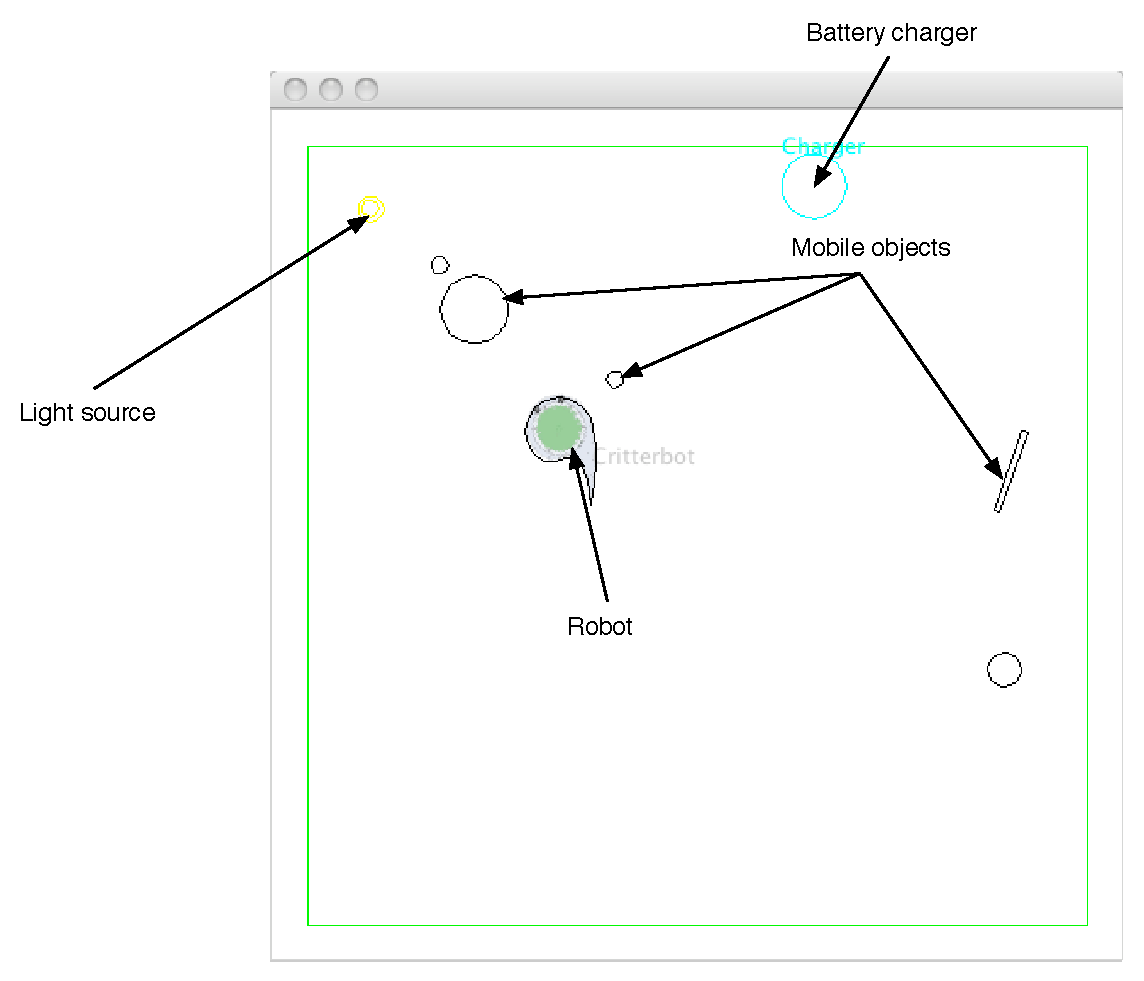
\psfig{file=images/Simulator_GUI.pdf,width=5in}
}
\caption{The RLAI Robotic Simulator Graphical User Interface.}
\end{figure}

You may find it inconvenient to recompile the source files every time. The
scripts provided in this package (including \code{runStandalone.sh}) take
command line arguments that modify the simulator behavior. In particular,
\code{-nc} will skip the compilation step and \code{-s} will specify a 
different time scale (with 1.0 being the default, and higher being faster)
at which the simulator should run. For example:

\begin{verbatim}
rlaisim/RLAIRobotSimulator/example> bash runStandalone.sh -nc -s 2.0
\end{verbatim}

will run the simulator without recompiling the source files in the
\code{example} directory and run at twice the real-time simulator speed.

\subsection{Running via RL-Glue}

The Standalone simulator does not actually require RL-Glue (in fact, you 
may have been able to proceed this far without even having RL-Glue installed).
However, if you downloaded this package you are most likely in doing some
kind of research. For simplicity, we provide an example agent, environment
and experiment which should allow you to quickly try out the Simulator.

The script \code{run.sh} will first compile the necessary source files (by
invoking \code{compile.sh}), then start, in turn:

\begin{enumerate}
\item{The environment (\code{SampleSimulatorEnvironment}, under \code{src/environment})}
\item{The agent (\code{RandomAgent}, under \code{src/agent})}
\item{The experiment (\code{SampleExperiment}, under \code{src/experiment})}
\item{RL-Glue (installed as the RL-Glue core)}
\end{enumerate}

If the RL-Glue core is not installed or the corresponding executable 
\verb+rl_glue+ cannot be found, the script will nicely notify you and request
that you correct the situation.

The following will start everything: 

\begin{verbatim}
rlaisim/RLAIRobotSimulator/example> bash run.sh 
\end{verbatim}

After the script has started all four processes, it will then wait
for any of them to die, at which point it will attempt to terminate the rest. 

Once you start \verb+run.sh+, you should see a GUI appear (provided you are
running on a machine with a display), as in Standalone mode.
The arrow keys are disabled in Normal Mode to prevent competition for control 
between the agent and the user. In the RL-Glue version of the simulator,
events happen synchronously: the RL environment waits for an action from the
RL agent before executing the next step in the simulator.

\subsection{Interfacing with RL-Viz}

A separate utility, RL-Viz, can be used to run the RL-Glue version of the
simulator along with RL-Glue compatible agents. Although a full description
of RL-Viz and of the packaging method used by the RL-Library is beyond the 
scope of this tutorial, it is worth noting that it is relatively easy to 
create an RL-Viz compatible package.
In order to create a jar file usable by RL-Viz, you should add the
source files of interest to the \code{RLGlueSim/src} directory of the package.
It is recommended that files be put under directories corresponding to their
packages. In the case of the sample code provided, this implies copying the
files in \code{example/src/environment} to 
\code{RLGlueSim/src/org/rlcommunity/environments/rlaisim/examples}:

\begin{verbatim}
RLAIRobotSimulator> mkdir -p RLGlueSim/src/org/rlcommunity/environments/rlaisim/examples
RLAIRobotSimulator> cp example/src/environment/* 
  RLGlueSim/src/org/rlcommunity/environments/rlaisim/examples
\end{verbatim}

The ant script provided in the \code{RLGlueSim} is already configured to 
generate RL-Viz compatible jar files. In other words, after doing

\begin{verbatim}
RLAIRobotSimulator> cd RLGlueSim
RLAIRobotSimulator/RLGlueSim> ant build
\end{verbatim}

The file \code{RLGlueSim/products/RLGlueSim.jar} generated by the ant script
will be an RL-Viz compatible jar. Agent code may also be added to 
\code{RLGlueSim.jar} in this way, although it is recommended to make a separate
package.

In this section, we discussed how to install and run the package. We looked
into running either in Standalone mode or via RL-Glue. We also briefly
suggested how an RL-Viz package may be constructed. In the following section,
we will look into actually using the simulator - creating agents and
environments.

\section{Using the RLAI Robotic Simulator}

An RL-Glue project is usually composed of an environment, an agent and
an experiment. The specific description and purpose of each of these 
components may be found in the RL-Glue documentation. In this section, we
will discuss how to create the first two - the RL environment and the agent -
as well as how to modify the Simulator environment. The ``RL environment''
refers to the part of the system which interacts with the agen via the RL-Glue.
The ``Simulator environment'', on the other hand, refers to the components
of the simulator engine itself and to the objects that ``live'' in the
simulator. The RL environment is in charge of defining the action and 
observation space provided to the agent, whereas the Simulator environment
defines which objects are loaded and where they should initially be placed.

\subsection{Creating an Agent}

The sample agent provided with this package can be found under
\code{example/src/agent}. It simply is the random agent distributed with the 
RL-Library.

There are no specific restrictions as to the type of observations and 
actions that the agent should support. This is because the RL environment
defines the number and type of observations (and actions) that it provides.
Thus, the agent should match the style of observations and actions provided
by the environment. In our example, the actions come from a discrete 
one-dimensional set and the observation vector is composed of four real-valued 
features.

\subsection{Creating an RL Environment}

The package has been designed to abstract most of the simulator-related
aspects from the actual RL environment implementation. There are four 
components necessary to create a new environment:

\begin{enumerate}
\item{A \code{SimulatorActionMapping} that converts RL actions to commands to the robot in the simulator}
\item{A \code{SimulatorObservationMapping} that converts simulator observations into RL observations}
\item{A \code{SimulatorRewardFunction} that defines the reward function}
\item{An \code{EnvironmentDescription} that describes the Simulator environment}
\end{enumerate}

In the example provided in the package, the above components are instantiated
as \code{DiscreteActionMapping}, \code{LightSensorsObservationMapping},
\code{LightBasedRewardFunction} and \code{SampleSimulatorEnvironment},
respectively. A brief description of each follows; you are encouraged to
study the examples.

\subsubsection{DiscreteActionMapping (implements SimulatorActionMapping)}

This action mapping takes a discrete action (numbered between 0 and 5) and
converts it into movement along one of the robot's three degrees of freedom.
Actions 0 and 1 move forward and backward, while actions 2 and 3 move
laterally and actions 4 and 5 rotate the robot. This is possible because the
Critterbot is designed with an omnidirectional drive.

The job of the \code{SimulatorActionMapping} is to return a 
\code{CritterControlDrop} (this may be a different class if a different
robot interface is used, but this is beyond the scope of this section).
The \code{CritterControlDrop} encapsulates a command sent to the Critterbot
in the Simulator. The \code{DiscreteActionMapping} simply sets one of the
three important variables in \code{CritterControlDrop} - \verb+x_velocity+,
\verb+y_velocity+ or \verb+theta_velocity+ - to specify how the robot
should move. Each velocity may be specified independently.

As an additional example, you may wish to try making the actions 
non-orthogonal by adding a rotational component to actions 0 to 3 and a
translational component to actions 4 and 5.

A \code{SimulatorActionMapping} must also provide range information about the
allowed RL actions. 

The Javadocs on the CritterControlDrop describes the different fields
that may be set.

\subsubsection{LightSensorsObservationMapping (implements SimulatorObservationMapping)}

An observation mapping takes a Simulator drop containing observation 
information (in the case of the Critterbot, this is a CritterStateDrop)
and converts it into an RL-Glue observation.  This particular mapping simply
returns a four-dimensional observation vector, composed of the four light
sensor values on the Critterbot - bounded to be within the allowed range.

As an additional example, you may wish to include infrared distance sensor
information in the observation vector. The array \verb+ir_distance+ of the
\code{CritterStateDrop} contains the sensor values for the IR distance
sensors on the simulated Critterbot.

Like a \code{SimulatorActionMapping}, a \code{SimulatorObservationMapping}
implementer must provide methods returning the ranges of values that its
observation features may take.

The Javadocs on the CritterStateDrop describes the various sensor readings
generated by the simulator.

\subsubsection{LightBasedRewardFunction (implements SimulatorRewardFunction)}

A reward function, as one may expect, maps state-action-state transitions to
a reward value. In the case of the \code{LightBasedRewardFunction}, the 
reward is 1.0 if the front light sensor (corresponding to the next state's
first observation feature) reports a value greater or equal to 400. Otherwise,
the returned reward is 0. Thus, this reward function encodes that being close
to a light source and facing it is good.

As an additional example, you may want to give negative reward to a robot
which has low (or no) battery power. This can be done by adding battery 
information, found under the fields \verb+batv40+, \verb+batv160+ and
\verb+batv280+ in the \code{CritterStateDrop}.

Similar to the \code{SimulatorActionMapping} and 
\code{SimulatorObservationMapping}, a \code{SimulatorRewardFunction}
implementer must provide a range for its reward function.

\subsubsection{SampleSimulatorEnvironment (implements EnvironmentDescription)} 

The \code{EnvironmentDescription} interface (from the core Simulator library)
provides methods for describing a Simulator environment. A class which 
implements \code{EnvironmentDescription} must provide a method,
\code{generateObjects}, which returns the list of objects present in the
Simulator. As a rule of thumb, everything in the Simulator is an object:
the walls surrounding the world, the movable balls and bars in the
environment, the robot itself... The class \code{CommonObjects} (also from
the core Simulator library) provides a set of methods meant for easily
creating new objects.

As an additional example, you may want to add a second light source to the
sample Simulator environment.

\subsubsection{Putting it all together}

The sample RL environment extends the abstract class 
\code{AbstractSimulatorEnvironment}. Calling the latter's constructor 
appropriately and implementing its abstract methods is what is needed
to obtain a complete RL environment.

The three first components described above - the observation mapping, the
action mapping and the reward function - are all provided to the 
constructor of \code{AbstractSimulatorEnvironment}. Furthermore, the
following methods must be implemented:

\begin{itemize}
\item{\code{getEnvironmentDescription} - should return the fourth of the above components.}
\item{\code{addEngineComponents} - this method is in charge of adding the necessary SimulatorComponents. The latter are, as the name implies, functional parts of the Simulator - for example, light sources and sensors require \code{SimulatorComponentLight}.}
\item{\code{getDiscountFactor} - returns the discount factor for this environment.}
\item{\code{isTerminal} - returns whether the environment has reached a terminal state.}
\end{itemize}

\end{document}
